\documentclass{report}
\usepackage{float}
\usepackage{graphicx}
\usepackage{amsmath}
\usepackage{listings}
\usepackage{xcolor}
\lstset{
	upquote=true,
	basicstyle=\ttfamily\footnotesize,
	language=C,
	keywordstyle=\color{magenta},
	showstringspaces=false,
	tabsize=2,
	backgroundcolor=\color{blue!15},
}

\begin{document}
	\title{\LaTeX Tutorial}
	\author{Arjun C}
	\maketitle
	\tableofcontents
	\listoffigures
	\chapter{Sachin Tendulkar}
	\section{Introduction}
Sachin Ramesh Tendulkar (born 24th April 1973) is a former Indian international cricketer and a former captain of the Indian national team, regarded as one of the greatest batsman of all time. He is the highest run scorer of all time in International cricket. Tendulkar took up cricket at the age of eleven, made his Test debut on 15 November 1989 against Pakistan in Karachi at the age of sixteen, and went on to represent Mumbai domestically and India internationally for close to twenty-four years. He is the only player to have scored one hundred international centuries, the first batsman to score a double century in a ODI, the holder of the record for the most number of runs in both Test and ODI, and the only player to complete more than 30,000 runs in international cricket. He is colloquially known as Little Master or Master Blaster, and often referred to as the God of Cricket by Indian cricket followers. In 2001, Sachin Tendulkar became the first batsman to complete 10,000 ODI runs in his 259 innings. In 2002, halfway through his career, Wisden Cricketers' Almanack ranked him the second greatest Test batsman of all time, behind Don Bradman, and the second greatest ODI batsman of all time, behind Viv Richards. Later in his career, Tendulkar was a part of the Indian team that won the 2011 World Cup, his first win in six World Cup appearances for India. He had previously been named Player of the Tournament at the 2003 edition of the tournament, held in South Africa. In 2013, he was the only Indian cricketer included in an all-time Test World XI named to mark the 150th anniversary of Wisden Cricketers' Almanack. 

Tendulkar received the Arjuna Award in 1994 for his outstanding sporting achievement, the Rajiv Gandhi Khel Ratna award in 1997, India's highest sporting honour, and the Padma Shri and Padma Vibhushan awards in 1999 and 2008, respectively, India's fourth and second highest civilian awards. After a few hours of his final match on 16 November 2013, the Prime Minister's Office announced the decision to award him the Bharat Ratna, India's highest civilian award. He is the youngest recipient to date and the first ever sportsperson to receive the award. He also won the 2010 Sir Garfield Sobers Trophy for cricketer of the year at the ICC awards. In 2012, Tendulkar was nominated to the Rajya Sabha, the upper house of the Parliament of India. He was also the first sportsperson and the first person without an aviation background to be awarded the honorary rank of group captain by the Indian Air Force. In 2012, he was named an Honorary Member of the Order of Australia.
\vspace{1cm}
In December 2012, Tendulkar announced his retirement from ODIs. He retired from Twenty20 cricket in October 2013 and subsequently retired from all forms of cricket on 16 November 2013 after playing his 200th Test match, against the West Indies in Mumbai's Wankhede Stadium. Tendulkar(Figure \ref{sachinface}) played 664 international cricket matches in total, scoring 34,357 runs.

"There are reports that m.."

\hfill{-Donald E. Knuth}

\section{More Info}
\begin{table}[H]
	\centering
\begin{tabular}{|l|c|c|r|}
	\hline
	\textbf{Type}&\textbf{Matches}&\textbf{Runs}&\textbf{Avg.}\\
	\hline \hline
	Test&200&15921&53.78\\
	\hline 
	ODI&463&5678&90 \\
	\hline
	ODI&463&5678&90 \\	
	\hline
\end{tabular}
\caption{Table 1 Test}
\label{cs}
\end{table}


\begin{table}[H]
	\centering
	\begin{tabular}{|l|c|c|r|}
		\hline
		\textbf{Type}&\textbf{Matches}&\textbf{Runs}&\textbf{Avg.}\\
		\hline \hline
		Test&200&15921&53.78\\
		\hline 
		ODI&463&5678&90 \\
		\hline
		ODI&463&5678&90 \\	
		\hline
	\end{tabular}
	\caption{Table 1 Test}
\end{table}
\subsection{Pics}
\begin{figure}
	\centering
	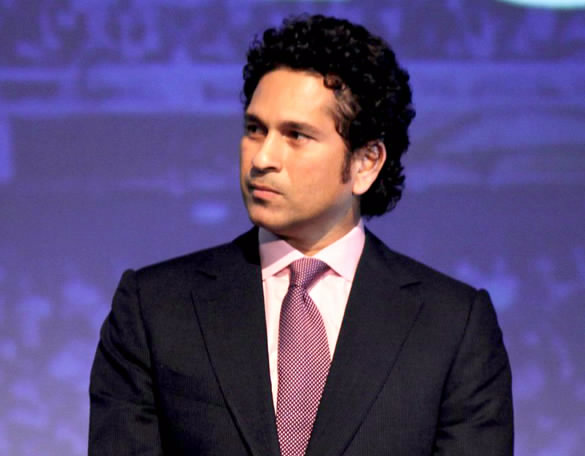
\includegraphics[scale=0.5]{Sachin-01}
	\label{sachinface}
	\caption{Sachin Tendulkar}

\end{figure}

\begin{figure}
	\centering
	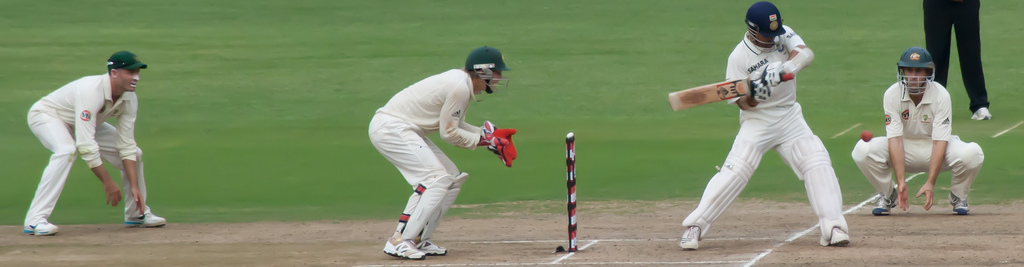
\includegraphics[scale=0.40]{Sachin-02}
	\label{sachinface}
	\caption{Sachin Tendulkar}
	
\end{figure}

National Awards
\begin{enumerate}
	\item National Awards
	\item Arjuna Award
		\begin{itemize}
			\item 1997
			\item 1996
		\end{itemize}
	\item Padma Shri
	\item Padma Vibhushan
	\item Bharat

\end{enumerate}


\chapter{Mathemathics}

The general form of a quadratic equation is $ax^2+bx+c=0$. Where  $a$ is coefficent of $x^2$ and $c$ is a constant

The general form of quadratic equation is 
\begin{displaymath}
	ax^2+bx+c=0
\end{displaymath}
Where  $a$ is coefficent of $x^2$ and $c$ is a constant


Testing equation env.

\begin{equation}
	ax^3+bx+c=0
\end{equation}
Where  $a$ is coefficent of $x^2$ and $c$ is a constant


\begin{equation}
	ax^2+bx+c=0
\end{equation}
Where  $a$ is coefficent of $x^2$ and $c$ is a constant



\begin{equation}
	\cos 2\theta = \cos^2\theta - \sin^2\theta
\end{equation}

\begin{equation}
	\lim_{x \to \infty} \exp(-x) = 0
\end{equation}

\begin{equation}
	\frac{n!}{k!(n-k)!} = \binom{n}{k} 
\end{equation}

\begin{equation}
	\frac{sinX}{n} = siX = 6
\end{equation}

\begin{equation}
	\frac{\frac{1}{x}+\frac{1}{y}}{y-z}
\end{equation}

\begin{equation}
	\sqrt{\frac{z}{y}}
	\sqrt[n]{1+x+x^2+x^3+\ldots}
\end{equation}

\begin{equation}
	\sum_{i=1}^{10} t_i
\end{equation}

\begin{equation}
	\int_0^\infty \mathrm{e}^{-x}\,\mathrm{d}x
\end{equation}

Roots of a quadratic quation are
\begin{equation}
	\frac{-b \pm \sqrt{b^2-4ac}}{2a}
\end{equation}
	
	
\chapter{Introduction to C}
\begin{lstlisting}[caption={Program to check odd or even}]
#include<stdio.h>
int main()
{
	int a;
	printf("Enter a number: ");
	scanf("%d", &a);
	if(a%2 == 0)
	{
		printf("%d is an even number", a);
	}
	else
	{
		printf("%d is an odd number", a);
	}
}
\end{lstlisting}


Tendulkar was born at Nirmal Nursing Home in Dadar, Bombay on 24 April 1973 to a Maharashtrian Rajapur Saraswat Brahmin family. His father, Ramesh Tendulkar, was a well-known Marathi novelist \& poet and his mother, Rajni, worked in the insurance industry. Ramesh named Tendulkar after his favourite music director, Sachin Dev Burman. Tendulkar has three elder siblings: two half-brothers Nitin and Ajit, and a half-sister Savita. They were Ramesh's children by his first wife, who died after the birth of her third child.

Tendulkar spent his formative years in the Sahitya Sahawas Cooperative Housing Society in Bandra (East). As a young boy, Tendulkar was considered a bully, and often picked up fights with new children in his school. He also showed an interest in tennis, idolising John McEnroe. To help curb his mischievous and bullying tendencies, Ajit introduced the young Sachin to cricket in 1984. He introduced him to Ramakant Achrekar, a famous cricket coach and a club cricketer of repute, at Shivaji Park, Dadar. In the first meeting, the young Sachin did not play his best. Ajit told Achrekar that he was feeling self-conscious due to the coach observing him, and was not displaying his natural game. Ajit requested the coach to give him another chance at playing, but watch while hiding behind a tree. This time, Sachin, apparently unobserved, played much better and was accepted at Achrekar's academy.

Achrekar was impressed with Tendulkar's talent and advised him to shift his schooling to Sharadashram Vidyamandir (English) High School, a school at Dadar which had a dominant cricket team and had produced many notable cricketers. Prior to this, Tendulkar had attended the Indian Education Society's New English School in Bandra (East). He was also coached under the guidance of Achrekar at Shivaji Park in the mornings and evenings. Tendulkar would practice for hours on end in the nets. If he became exhausted, Achrekar would put a one-rupee coin on the top of the stumps, and the bowler who dismissed Tendulkar would get the coin. If Tendulkar passed the whole session without getting dismissed, the coach would give him the coin. Tendulkar now considers the 13 coins he won then as some of his most prized possessions. He moved in with his aunt and uncle, who lived near Shivaji Park, during this period, due to his hectic schedule.










\end{document}
